% TODO: Para cada modelo colocar como que é a entrada na forma de uma expressão matemática

\section{Tráfego}


\section{\acrfull{NN}}


\section{\acrfull{RNN}}

% RESOURCE: to explain recurrent neural networks (http://d2l.ai/chapter_recurrent-neural-networks/index.html)

% TODO: Falar que nem todos os dados são independentes, então a RNN serve para lembrar de alguns dados que já passaram pelo modelo para melhorar a performance.

% TODO: Falar que é melhor para predição aparentemente (pode ser algo a ver com o tipo de dados que temos)

% TODO: Falar que sofre de memória curta e outros defeitos

% TODO?: Falar que basicamente é um modelo feito para lidar com dados dependentes

\section{\acrfull{LSTM}}

\acrshort{LSTM} é amplamente utilizado para predição de tráfego e de informações que derivam de dados sequenciais/séries temporais, sendo possível encontrar diversos trabalhos na literatura que mostram sua eficiência quando comparado a outros métodos. Como descrito em \cite{Zainab_2018} e em \cite{Xiaolei_2015}, \acrshort{LSTM} é um tipo de \acrfull{RNN} que utiliza de estados anteriores e do estado atual da rede para gerar sua saída. Ao utilizar dos estados anteriores, a \acrshort{RNN} acaba por simular uma memória, melhorando seu aprendizado. 

\begin{figure}[htb]
    \centering
    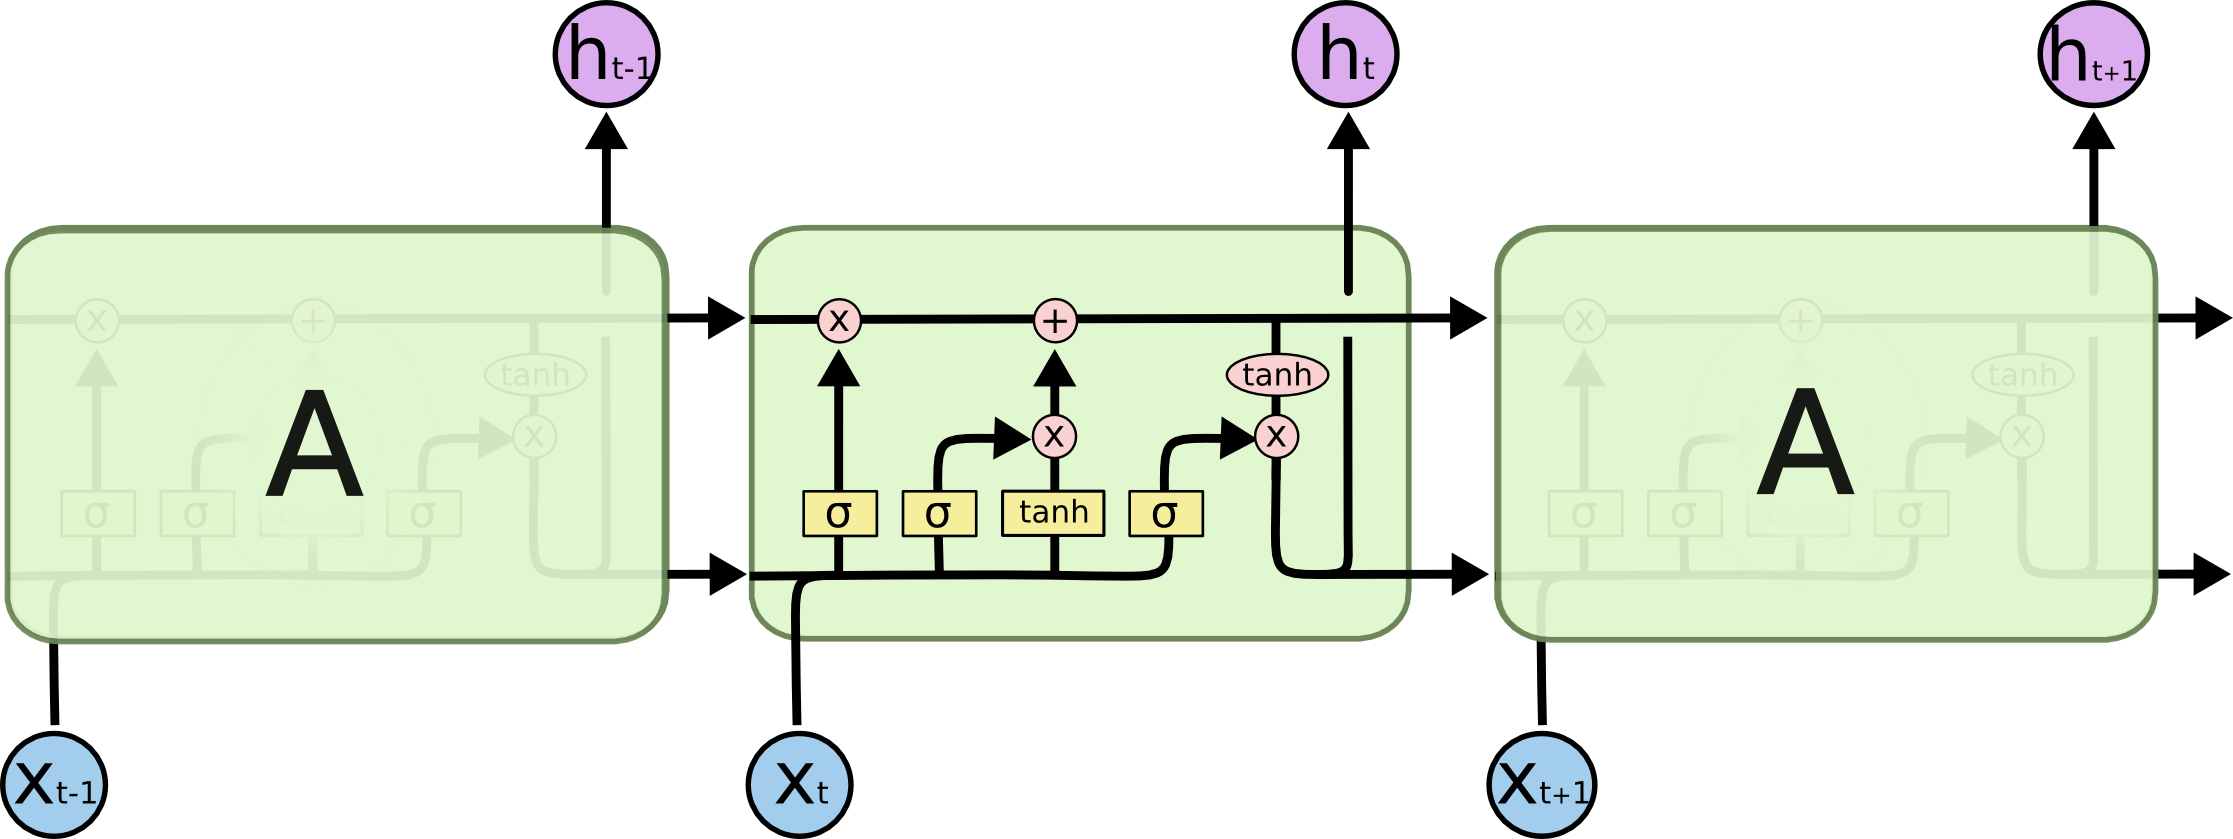
\includegraphics[scale=0.4]{lstm3.png}
    \label{figure:eixo}
    \caption[Representação de uma arquitetura LSTM]{Representação de uma arquitetura LSTM\footnotemark}
\end{figure}

\footnotetext{https://colah.github.io/posts/2015-08-Understanding-LSTMs/}

Porém, diferentemente de uma \acrshort{RNN}, o LSTM possui uma unidade a mais em seus blocos chamada de célula de memória. Esta célula é capaz de perceber as características mais latentes dos dados e descartar as menos importantes. Assim, o \acrshort{LSTM} consegue manter as características mais importantes na rede por mais tempo que uma \acrfull{RNN} comum. Por estes motivos, o \acrshort{LSTM} é excelente para modelar séries temporais e dados sequenciais.

Nesta célula de memória existem estruturas que são responsáveis pela característica de memória a longo prazo do \arcshort[LSTM]. A Porta de Entrada, a Porta do esquecimento e a Porta de Saída. Abaixo, explicaremos como cada um deles funciona:

\begin{itemize}
  \item Porta de Entrada: 
  \item Porta do Esquecimento: 
  \item Porta de Saída:
\end{itemize}

% TODO: Falar que podemos responder a quantidade de camadas da LSTM com o problema que RNN tem com back-propagation que o gradiente começa a diminuir exponencialmente. Mas tem que dar uma conferida melhor.

\section{\acrfull{GRU}}

\section{\acrfull{RF}}

\textit{\acrshort{RF}} é em uma união de métodos, no caso, é uma união de diversas árvores de decisão. Então para se entender \textit{\acrshort{RF}} é preciso primeiro entender árvores de decisão.

\subsection{Árvores de Decisão}



\section{\acrfull{SVM}}

% RESOURCE: to learn better how random forest work (https://stackabuse.com/random-forest-algorithm-with-python-and-scikit-learn/)

